
\section{O HARDWARE DO ROBÔ}

Após o contato com outras equipes e pesquisa em relação aos materiais, decidiu-se por reformular a estrutura dos robôs. Visando a simplificação das montagens, bem como agilidade na manutenção, os robôs adquiriram um escopo modular. Dessa forma, cada conjunto de componentes responsável por um setor do robô é acoplado a um dos módulos separadamente. Assim, caso algum dos módulos apresente problemas de execução, ele pode ser trocado por outro igual reserva, sem que haja excessiva perda de tempo. Inicialmente, cogitou-se a existência de três módulos: os motores junto das rodas; a bateria; e a placa controladora com os componentes discretos. O módulo da placa controladora, que contém, entre outros componentes, o Arduino Nano[6], é agora livre de fios e componentes soldados diretamente ao fenolite. Novamente em busca de agilidade na manutenção, somente soquetes e caixas de pinos foram soldadas diretamente na placa, de modo que os componentes são removíveis e de fácil substituição. A bateria, que é empregada agora no lugar das pilhas AA de versões anteriores, ocupa sozinha, junto de um pequeno circuito de verificação de carga, o segundo módulo. Isso ocorre devido ao trabalho necessário para carregá-la. Diferentemente das pilhas, onde bastava uma fonte de alimentação para recarregar o robô, a bateria de lítio exige um circuito próprio externo ao robô para carregar adequadamente. O circuito verificador de carga é responsável por impedir que a bateria chegue a níveis muito baixos, o que prejudicaria seu desempenho. O último dos módulos é composto pelos motores e rodas. A única diferença desse sistema para o anterior é o diâmetro das rodas, que cresceu 2mm, e seu acabamento.

% FIGURA
\begin{figure}[!htb]
\centering
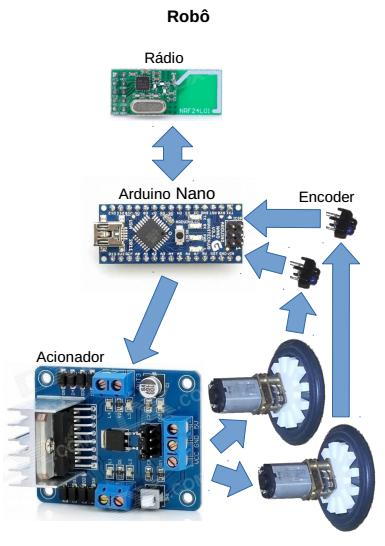
\includegraphics[scale=0.7]{hardware_robo.png}
\caption{Esquema dos componentes eletrônicos usados em cada robô.}
\label{fig:hardware_robo}
\end{figure}

O robô foi construído tem um Arduino Nano[6] como módulo de controle. Este módulo recebe, via um transceptor de rádio NRF24L01, os comandos de velocidade desejados para cada uma das rodas. O Arduino aciona os motores utilizando modulação por largura de pulso PWM (Pulse-Width Modulation) através de uma placa equipada com o componente por um circuito impresso L293.

A rotação das rodas, e consequentemente o deslocamento do robô, são determinados por sensores TCRT5000, que codificam o movimento de dentes reflexivos fixados às rodas em pulsos enviados ao Arduino. Esses pulsos são contados e servem de realimentação ao acionamento direcionado a cada motor. Um esquema representativo da eletrônica do robô pode ser apreciado na Fig. \ref{fig:hardware_robo} .

Do lado do computador pessoal, o envio dos comandos também ocorre através de um circuito controlado por um Arduino Nano[6] conectado a uma interface USB. Este Arduino recebe os comandos a ser enviados aos robôs e os transmite por meio de um transceptor de rádio NRF24L01 idêntico ao utilizados nos robôs.
